% généré depuis source/08_validation.md — ne pas modifier à la main
\chapter{Validation et résultats}\label{sec:resultats}

\chapintro

Ce chapitre présente le protocole expérimental et les métriques, puis les résultats obtenus pour la fiabilité, la maintenabilité et la disponibilité, la détection de l'état critique et l'estimation de la durée de vie résiduelle, avant de comparer les méthodes. Tous les chiffres de ce chapitre proviennent des fichiers de résultats produits par \code{run\_all.py} ; les figures et les tableaux sont générés à partir de ces fichiers.

\section{Protocole expérimental et métriques}\label{sec:protocole}

\subsection{Découpages des données et validation}\label{sec:decoupages}

Le découpage officiel de FD001 est respecté : les modèles sont appris sur les 100 moteurs d'entraînement et évalués sur les 100 moteurs de test, jamais vus pendant l'apprentissage. Les choix propres à chaque partie sont les suivants :

\begin{itemize}
\item \textbf{fiabilité} : population de 200 unités, avec 100 défaillances et 100 censures à droite (section~\ref{sec:donnees-censure}) ; le RUL réel des moteurs de test n'est pas utilisé ;
\item \textbf{classification} : validation croisée par groupes de moteurs (5 plis) sur l'entraînement, puis évaluation sur \textbf{tous les cycles} des moteurs de test ;
\item \textbf{RUL} : évaluation au \textbf{dernier cycle observé} de chaque moteur de test, comme dans le challenge PHM \cite{saxena2008damage} ; le LSTM réserve 15 moteurs d'entraînement à l'arrêt précoce.
\end{itemize}

\subsection{Métriques}\label{sec:metriques}

\textbf{Fiabilité.}

Le test de Kolmogorov-Smirnov accepte une loi si sa \emph{p}-valeur dépasse $\alpha = 5\,\%$. L'AIC compare les lois entre elles, et le coefficient $R^2$ mesure la linéarité du diagramme de Weibull (section~\ref{sec:fiabilite}).

\textbf{Classification.}

Avec $VP$, $FP$, $VN$ et $FN$ les vrais et faux positifs et négatifs (la classe positive étant l'état critique), on utilise :

\begin{equation}\label{eq:classif}
\text{précision} = \frac{VP}{VP + FP}, \qquad \text{rappel} = \frac{VP}{VP + FN}, \qquad F_1 = \frac{2\,\text{précision} \cdot \text{rappel}}{\text{précision} + \text{rappel}}.
\end{equation}

En maintenance, le \textbf{rappel} est la métrique la plus importante, car une défaillance manquée coûte bien plus cher qu'une inspection inutile. L'aire sous la courbe ROC (AUC) \cite{hanley1982} mesure la capacité à classer un cycle critique au-dessus d'un cycle normal, indépendamment du seuil de décision.

\textbf{Durée de vie résiduelle.}

L'erreur d'un moteur est $e_i = \widehat{\mathrm{RUL}}_i - \mathrm{RUL}_i$ : une erreur \textbf{positive} est une prédiction \textbf{tardive}, la plus dangereuse puisqu'elle annonce plus de vie qu'il n'en reste. Sur les $N$ moteurs de test :

\begin{equation}\label{eq:rmse}
\mathrm{RMSE} = \sqrt{\frac1N \sum_i e_i^2}, \qquad \mathrm{MAE} = \frac1N \sum_i |e_i|, \qquad \text{biais} = \frac1N \sum_i e_i .
\end{equation}

Le \textbf{score NASA} \cite{saxena2008damage} pénalise exponentiellement les erreurs, et davantage les prédictions tardives :

\begin{equation}\label{eq:score}
S = \sum_i s_i, \qquad s_i = \begin{cases} e^{-e_i/13} - 1 & e_i < 0 \\ e^{e_i/10} - 1 & e_i \ge 0 \end{cases}.
\end{equation}

Pour le modèle de dégradation, la qualité de l'incertitude est mesurée par la \textbf{couverture empirique} : la proportion de moteurs dont le RUL réel tombe dans l'intervalle de prédiction. Un intervalle bien calibré de niveau nominal $q$ couvre le RUL réel dans une proportion proche de $q$ ; une couverture inférieure signale une incertitude sous-estimée. Trois niveaux sont évalués : P25–P75, P10–P90 et P05–P95.

\section{Fiabilité}\label{sec:res-fiabilite}

\subsection{Estimation non paramétrique}

La courbe de Kaplan-Meier (figure~\ref{fig:fiabilite_kaplan_meier}) vaut un jusqu'à la première défaillance, puis décroît rapidement. La médiane de survie est de 202 cycles et l'aire sous la courbe de 214,3 cycles. Les censures (moteurs de test) se concentrent aux faibles âges, où presque toute la population est encore à risque ; elles élargissent peu l'intervalle de confiance, qui ne s'ouvre vraiment qu'aux grands âges, quand peu de moteurs restent à risque.

\begin{figure}[htbp]
\centering
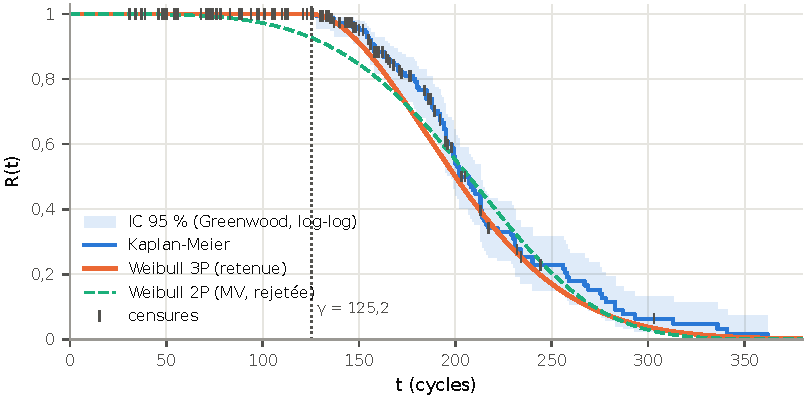
\includegraphics[width=1\linewidth]{figures/fiabilite_kaplan_meier.pdf}
\caption{Fonction de fiabilité : estimateur de Kaplan-Meier avec son intervalle de confiance et les censures, comparé à la loi de Weibull 3P retenue et à la loi de Weibull 2P (MV) rejetée.}\label{fig:fiabilite_kaplan_meier}
\end{figure}

Le taux de défaillance estimé par Nelson-Aalen (figure~\ref{fig:fiabilite_taux_defaillance}) est nul jusqu'à l'âge de la première défaillance, puis croît : c'est la signature d'une \textbf{usure}. Ses oscillations aux grands âges reflètent le faible nombre de moteurs encore à risque et non un phénomène physique.

\begin{figure}[htbp]
\centering
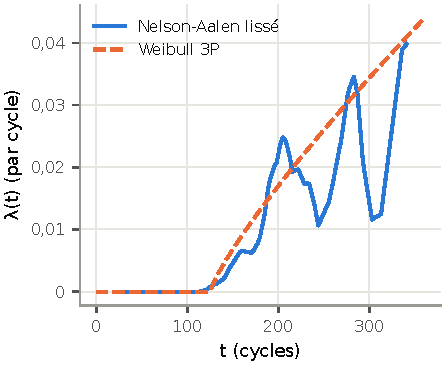
\includegraphics[width=1\linewidth]{figures/fiabilite_taux_defaillance.pdf}
\caption{Taux de défaillance : estimation non paramétrique de Nelson-Aalen lissée par noyau et taux de la loi de Weibull 3P.}\label{fig:fiabilite_taux_defaillance}
\end{figure}

\subsection{Choix de la loi}

Le tableau~\ref{tab:fiabilite_modeles} et le tableau~\ref{tab:fiabilite_adequation} résument les ajustements. Le diagramme de Weibull (figure~\ref{fig:fiabilite_diagramme_weibull}) est nettement \textbf{courbé} : les points s'écartent de la droite aux deux extrémités et le coefficient de détermination ne vaut que 0,894. La pente donne $\beta = 5{,}52$ par MCO. L'estimation par MV de la loi de Weibull 2P sur les défaillances donne $\beta = 4{,}41$, mais elle est \textbf{rejetée} par le test de Kolmogorov-Smirnov ($p = 0{,}013$). Avec la censure, l'estimation sur les 200 unités donne $\beta = 4{,}82$ (intervalle de confiance $[4{,}22 ; 5{,}42]$) et $\eta = 236{,}6$ cycles : l'échelle est plus grande, car les moteurs censurés apportent l'information qu'ils ont survécu au moins jusqu'à leur dernier cycle observé.

\begin{figure}[htbp]
\centering
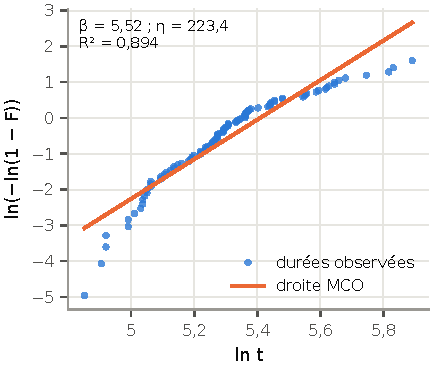
\includegraphics[width=0.55\linewidth]{figures/fiabilite_diagramme_weibull.pdf}
\caption{Diagramme de Weibull (rangs médians de Bernard) et droite des moindres carrés : la courbure révèle un paramètre de position non nul.}\label{fig:fiabilite_diagramme_weibull}
\end{figure}

\begin{table}[htbp]
\centering\small
\begin{adjustbox}{max width=\linewidth,center}
\begin{tabular}{lrrrll}
\toprule
Méthode & \ensuremath{\beta} & \ensuremath{\eta} (cycles) & \ensuremath{\gamma} (cycles) & Adéquation & Décision \\
\midrule
Weibull 2P, MCO (rangs de Bernard) & 5,52 & 223,4 & 0 & R\textsuperscript{2} = 0,894 & diagramme courbé \\
Weibull 2P, MV & 4,41 & 225,0 & 0 & KS p = 0,013 & rejetée \\
Weibull 2P, MV avec censure (200 unités) & 4,82 [4,22 ; 5,42] & 236,6 & 0 & — & comparaison \\
\textbf{Weibull 3P, MV} & \textbf{1,83} & \textbf{91,3} & \textbf{125,2} & KS p = 0,32 & \textbf{retenue} \\
\bottomrule
\end{tabular}
\end{adjustbox}
\caption{Modèles de fiabilité estimés sur les 100 durées de défaillance}\label{tab:fiabilite_modeles}
\end{table}

\begin{table}[htbp]
\centering\small
\begin{adjustbox}{max width=\linewidth,center}
\begin{tabular}{lrrrrrl}
\toprule
Loi & Paramètres & Log-vraisemblance & AIC & KS D & KS p & Décision (\ensuremath{\alpha} = 5 \%) \\
\midrule
Exponentielle & 1 & \ensuremath{-}632,94 & 1\,267,88 & 0,470 & 0,000 & rejetée \\
Weibull 2P & 2 & \ensuremath{-}530,75 & 1\,065,50 & 0,157 & 0,013 & rejetée \\
Log-normale & 2 & \ensuremath{-}517,46 & 1\,038,91 & 0,094 & 0,317 & acceptée \\
Weibull 3P & 3 & \ensuremath{-}516,52 & 1\,039,03 & 0,094 & 0,319 & acceptée \\
\bottomrule
\end{tabular}
\end{adjustbox}
\caption{Adéquation des lois candidates (MV sur les durées complètes)}\label{tab:fiabilite_adequation}
\end{table}

La loi exponentielle est rejetée sans ambiguïté ($p = 0{,}000$, AIC 1\,267,88), ce qui exclut un taux de défaillance constant. Les lois de Weibull 3P (AIC 1\,039,03, $p = 0{,}32$) et log-normale (AIC 1\,038,91, $p = 0{,}32$) sont toutes deux acceptées, avec une différence d'AIC de 0,12 seulement : elles sont \textbf{statistiquement équivalentes}, et toutes deux bien meilleures que la loi de Weibull 2P (AIC 1\,065,50). La loi de \textbf{Weibull 3P est retenue} pour trois raisons :

\begin{enumerate}
\item son paramètre de position $\gamma = 125{,}2$ cycles a une interprétation physique directe, la durée de fonctionnement sans défaillance garantie, cohérente avec la première défaillance observée à 128 cycles ;
\item son paramètre de forme $\beta = 1{,}83 > 1$ traduit un taux de défaillance croissant, conforme à l'estimation non paramétrique ;
\item elle est la loi de référence du cours et de la fiabilité mécanique \cite{benhmida,weibull1951}.
\end{enumerate}

\subsection{Indicateurs de fiabilité}

Le tableau~\ref{tab:fiabilite_indicateurs} donne les indicateurs du modèle retenu : MTTF de 206,3 cycles, $B_1 = 132{,}6$, $B_{10} = 151{,}9$ et $B_{50} = 199{,}9$ cycles. La durée $B_{50}$ est proche de la médiane de Kaplan-Meier (202 cycles), ce qui confirme l'accord entre les deux approches au centre de la distribution. La densité et la fonction de répartition (figure~\ref{fig:fiabilite_densite_repartition}) montrent une distribution concentrée entre la fin de la période sans défaillance et les âges de l'ordre de trois cents cycles.

\begin{table}[htbp]
\centering\small
\begin{adjustbox}{max width=\linewidth,center}
\begin{tabular}{lrl}
\toprule
Indicateur & Valeur & Source \\
\midrule
MTTF = \ensuremath{\gamma} + \ensuremath{\eta}·\ensuremath{\Gamma}(1 + 1/\ensuremath{\beta}) & 206,3 cycles & Weibull 3P \\
B1 (1 \% de défaillances) & 132,6 cycles & Weibull 3P \\
B10 (10 \%) & 151,9 cycles & Weibull 3P \\
B50 (médiane) & 199,9 cycles & Weibull 3P \\
Médiane de survie & 202 cycles & Kaplan-Meier \\
Aire sous la courbe de survie & 214,3 cycles & Kaplan-Meier \\
Première défaillance observée & 128 cycles & données \\
\bottomrule
\end{tabular}
\end{adjustbox}
\caption{Indicateurs de fiabilité}\label{tab:fiabilite_indicateurs}
\end{table}

\begin{figure}[htbp]
\centering
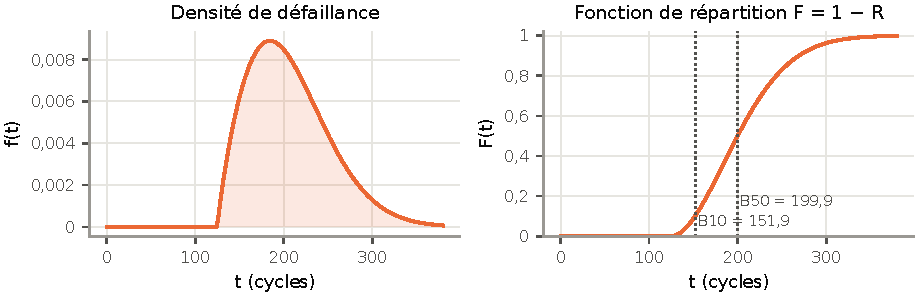
\includegraphics[width=1\linewidth]{figures/fiabilite_densite_repartition.pdf}
\caption{Densité de défaillance et fonction de répartition de la loi de Weibull 3P, avec les durées B10 et B50.}\label{fig:fiabilite_densite_repartition}
\end{figure}

La fiabilité conditionnelle (figure~\ref{fig:fiabilite_conditionnelle}) vaut un tant que l'âge augmenté de l'horizon reste dans la période sans défaillance, puis décroît : un moteur âgé a une probabilité de plus en plus faible de franchir les 25 cycles suivants. Ce résultat justifie directement une politique de remplacement liée à l'âge.

\begin{figure}[htbp]
\centering
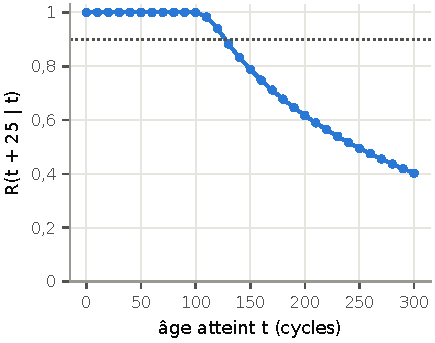
\includegraphics[width=0.55\linewidth]{figures/fiabilite_conditionnelle.pdf}
\caption{Fiabilité conditionnelle : probabilité qu'un moteur ayant atteint l'âge t fonctionne encore pendant l'horizon suivant (ligne pointillée : niveau $0{,}9$).}\label{fig:fiabilite_conditionnelle}
\end{figure}

\section{Maintenabilité, disponibilité et politique préventive}\label{sec:res-fmds02}

Ces résultats reposent sur les temps de réparation simulés (section~\ref{sec:fmds02}). La loi log-normale ré-estimée sur l'échantillon a pour paramètres $\mu = 2{,}742$ et $\sigma = 0{,}464$ ; le test de Kolmogorov-Smirnov l'accepte ($p = 0{,}61$). L'écart-type estimé est inférieur à la valeur utilisée pour la simulation (0,6) : c'est l'effet de la fluctuation d'échantillonnage sur un échantillon de cette taille. Le MTTR vaut 17,3 h, soit 8,6 cycles, et $90\,\%$ des réparations sont terminées en 28,1 h (figure~\ref{fig:fmds_maintenabilite}).

\begin{figure}[htbp]
\centering
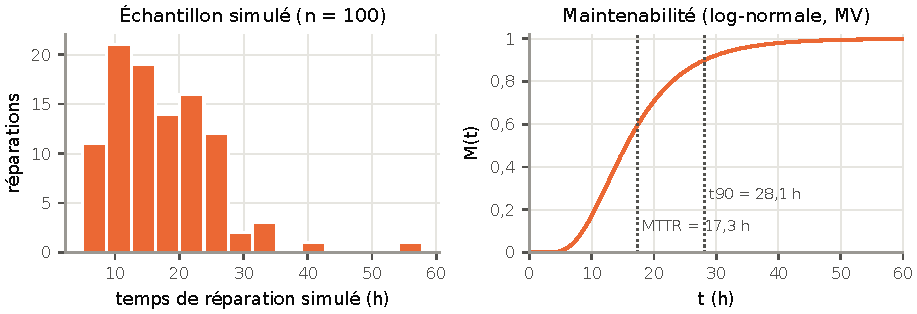
\includegraphics[width=1\linewidth]{figures/fmds_maintenabilite.pdf}
\caption{Temps de réparation simulés (gauche) et fonction de maintenabilité de la loi log-normale estimée, avec le MTTR et la durée t90 (droite).}\label{fig:fmds_maintenabilite}
\end{figure}

Le tableau~\ref{tab:fmds_maintenabilite_disponibilite} regroupe les indicateurs. La disponibilité intrinsèque vaut \textbf{95,98 \%}, soit environ 40,2 h d'indisponibilité pour mille heures. Selon le modèle markovien (figure~\ref{fig:fmds_disponibilite}), la disponibilité instantanée part de un et converge vers cette valeur en quelques dizaines de cycles.

\begin{table}[htbp]
\centering\small
\begin{adjustbox}{max width=\linewidth,center}
\begin{tabular}{ll}
\toprule
Grandeur & Valeur \\
\midrule
Loi des temps de réparation (MV) & log-normale, \ensuremath{\mu} = 2,742, \ensuremath{\sigma} = 0,464 (KS p = 0,61) \\
MTTR & 17,3 h = 8,6 cycles \\
t90 (90 \% des réparations terminées) & 28,1 h \\
MUT / MDT / MTBF & 206,3 / 8,64 / 215,0 cycles \\
Disponibilité intrinsèque A = MUT / (MUT + MDT) & 95,98 \% \\
Âge optimal de remplacement T* & 130,7 cycles, R(T*) = 0,994 \\
Coût par cycle : à T* / corrective seule & 0,0078 / 0,0242 (unités de Cp) \\
Gain du préventif & 67,7 \% \\
\bottomrule
\end{tabular}
\end{adjustbox}
\caption{Maintenabilité, disponibilité et remplacement préventif (temps de réparation simulés)}\label{tab:fmds_maintenabilite_disponibilite}
\end{table}

\begin{figure}[htbp]
\centering
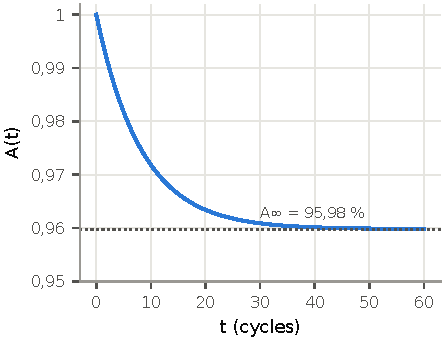
\includegraphics[width=0.55\linewidth]{figures/fmds_disponibilite.pdf}
\caption{Disponibilité instantanée A(t) selon le modèle markovien à deux états et sa limite asymptotique.}\label{fig:fmds_disponibilite}
\end{figure}

La politique de remplacement préventif (figure~\ref{fig:fmds_remplacement_preventif}) présente un optimum net à $T^* = 130{,}7$ cycles, juste après la fin de la période sans défaillance. À cet âge, la fiabilité vaut encore 0,994 : presque aucun moteur ne défaille en service. Le coût par cycle passe de 0,0242 (maintenance corrective seule) à 0,0078, soit une \textbf{réduction de 68 \%}. Le prix de ce gain est élevé : chaque moteur est remplacé en moyenne 75,6 cycles avant son MTTF.

\begin{figure}[htbp]
\centering
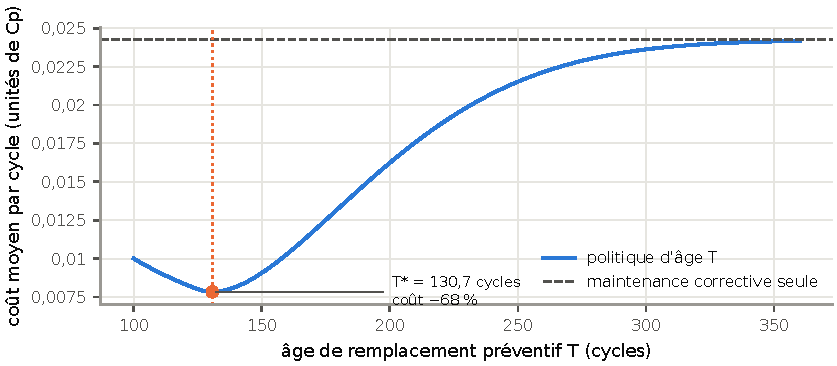
\includegraphics[width=1\linewidth]{figures/fmds_remplacement_preventif.pdf}
\caption{Coût moyen par cycle de la politique de remplacement à âge fixe en fonction de l'âge T, comparé au coût de la maintenance corrective seule.}\label{fig:fmds_remplacement_preventif}
\end{figure}

\section{Indicateur de santé et détection de l'état critique}\label{sec:res-sante}

\subsection{Sélection des capteurs et indicateur de santé}

Parmi les capteurs non constants, 12 présentent une tendance supérieure en valeur absolue au seuil de 0,5 et sont retenus : s2, s3, s4, s7, s8, s11, s12, s13, s15, s17, s20, s21 (figure~\ref{fig:sante_selection_capteurs}). Les capteurs s9 et s14, des vitesses de rotation du corps du moteur, ont une tendance plus faible et sont écartés.

\begin{figure}[htbp]
\centering
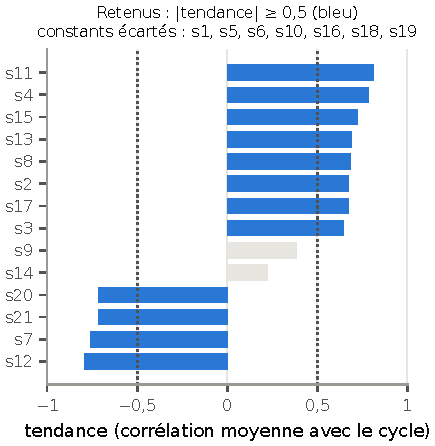
\includegraphics[width=0.55\linewidth]{figures/sante_selection_capteurs.pdf}
\caption{Tendance des capteurs non constants : corrélation moyenne avec le numéro de cycle ; les capteurs retenus dépassent le seuil en valeur absolue.}\label{fig:sante_selection_capteurs}
\end{figure}

L'indicateur de santé (figure~\ref{fig:sante_indicateur}) part d'environ un en début de vie et décroît jusqu'au voisinage de zéro à la défaillance, pour tous les moteurs, avec des durées de vie très différentes. Le seuil de défaillance appris par le modèle de dégradation vaut 0,002. Les poids de la combinaison linéaire (figure~\ref{fig:sante_poids_hi}) sont de signes opposés selon le sens de dérive des capteurs ; les plus forts portent sur la pression statique en sortie du compresseur haute pression (s11) et sur la température en sortie de la turbine basse pression (s4).

\begin{figure}[htbp]
\centering
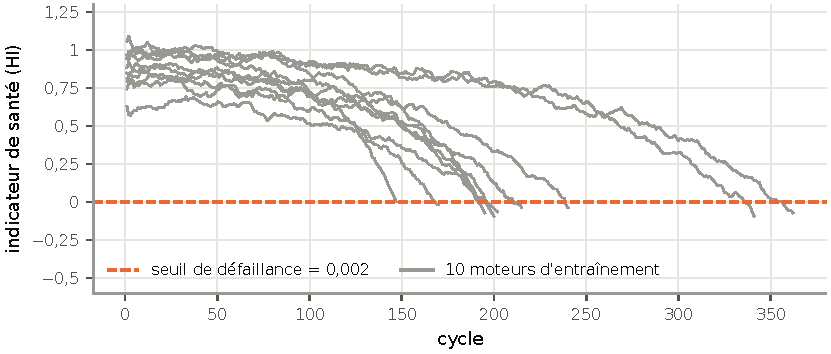
\includegraphics[width=1\linewidth]{figures/sante_indicateur.pdf}
\caption{Indicateur de santé lissé de dix moteurs d'entraînement et seuil de défaillance.}\label{fig:sante_indicateur}
\end{figure}

\begin{figure}[htbp]
\centering
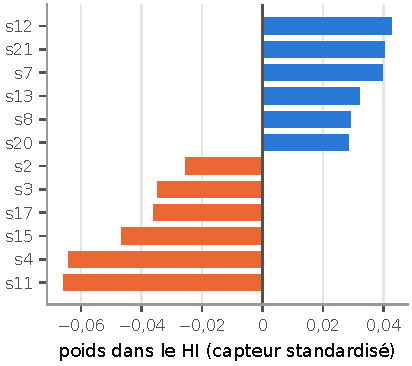
\includegraphics[width=0.55\linewidth]{figures/sante_poids_hi.pdf}
\caption{Poids des capteurs standardisés dans l'indicateur de santé.}\label{fig:sante_poids_hi}
\end{figure}

\subsection{Classification normal / critique}

Le tableau~\ref{tab:sante_classifieurs} présente les performances. Les deux classifieurs séparent très bien les deux classes : en validation croisée par groupes de moteurs, l'AUC vaut 0,990 pour le gradient boosting et 0,983 pour le SVM ; sur le jeu de test, 0,991 et 0,974 (figure~\ref{fig:sante_roc}). Le \textbf{gradient boosting} est retenu.

\begin{table}[htbp]
\centering\small
\begin{adjustbox}{max width=\linewidth,center}
\begin{tabular}{llrrrrr}
\toprule
Modèle & Évaluation & AUC & Exactitude & Précision & Rappel & F1 \\
\midrule
Gradient Boosting & validation croisée (GroupKFold 5) & 0,990 & 0,961 & 0,892 & 0,844 & 0,867 \\
 & test NASA & 0,991 & 0,986 & 0,747 & 0,657 & 0,699 \\
SVM (RBF) & validation croisée (GroupKFold 5) & 0,983 & 0,958 & 0,879 & 0,824 & 0,851 \\
 & test NASA & 0,974 & 0,986 & 0,798 & 0,621 & 0,698 \\
\bottomrule
\end{tabular}
\end{adjustbox}
\caption{Classification normal / critique (RUL \ensuremath{\le} 30 cycles)}\label{tab:sante_classifieurs}
\end{table}

\begin{figure}[htbp]
\centering
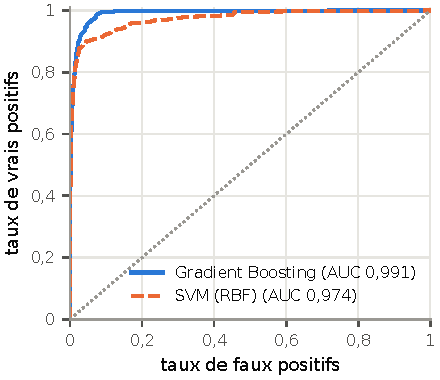
\includegraphics[width=0.55\linewidth]{figures/sante_roc.pdf}
\caption{Courbes ROC des deux classifieurs sur le jeu de test.}\label{fig:sante_roc}
\end{figure}

Au seuil de décision par défaut, le rappel de test est cependant nettement plus faible qu'en validation croisée (0,657 contre 0,844). La matrice de confusion (figure~\ref{fig:sante_matrice_confusion}) montre que, sur les 332 cycles critiques du jeu de test, 218 sont détectés et 114 manqués, pour 74 fausses alertes parmi 12\,690 cycles normaux correctement classés. Le jeu de test est très déséquilibré : la plupart des séries s'arrêtent bien avant la défaillance, et seuls les derniers cycles de quelques moteurs sont critiques. L'AUC élevée montre que le classement des probabilités reste bon ; c'est le \textbf{seuil} de décision qui est trop strict pour cet usage (section~\ref{sec:limites}).

\begin{figure}[htbp]
\centering
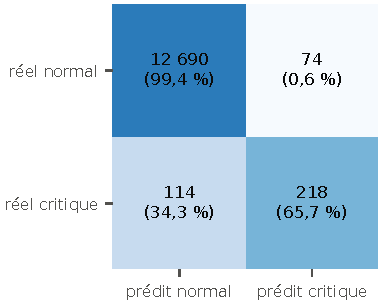
\includegraphics[width=0.50\linewidth]{figures/sante_matrice_confusion.pdf}
\caption{Matrice de confusion du gradient boosting sur le jeu de test, au seuil de décision par défaut.}\label{fig:sante_matrice_confusion}
\end{figure}

Au dernier cycle observé, la flotte de test se répartit en 76 moteurs normaux, 4 en surveillance et 20 critiques.

\section{Durée de vie résiduelle}\label{sec:res-rul}

\subsection{Performances des deux modèles}

Le tableau~\ref{tab:rul_metriques} compare les modèles sur les 100 moteurs de test. Le \textbf{LSTM est le plus précis} sur toutes les métriques : RMSE de 15,35 cycles contre 24,47, MAE de 11,22 contre 18,98, et score NASA de 485 contre 3\,743. Son biais est faible (+2,2 cycles), alors que le modèle de dégradation prédit en moyenne trop tard (+13,5 cycles, 78 \% de prédictions tardives). Le score NASA, qui pénalise fortement les retards, amplifie cet écart. La moyenne des deux prédictions (RMSE 16,91) n'améliore pas le LSTM seul : le biais du modèle de dégradation l'emporte sur le gain de la combinaison.

\begin{table}[htbp]
\centering\small
\begin{adjustbox}{max width=\linewidth,center}
\begin{tabular}{lrrrrrr}
\toprule
Modèle & RMSE & MAE & Biais & Score NASA & |e| \ensuremath{\le} 15 & Tardives \\
\midrule
Dégradation bayésienne (Eya) & 24,47 & 18,98 & +13,5 & 3\,743 & 49 \% & 78 \% \\
LSTM (Salma) & 15,35 & 11,22 & +2,2 & 485 & 68 \% & 58 \% \\
Moyenne des deux & 16,91 & 13,49 & +7,9 & 600 & 64 \% & 76 \% \\
\bottomrule
\end{tabular}
\end{adjustbox}
\caption{Performances des modèles de RUL sur les 100 moteurs de test}\label{tab:rul_metriques}
\end{table}

La figure~\ref{fig:rul_predit_vs_reel} montre les prédictions en fonction du RUL réel. Les prédictions du LSTM suivent la diagonale jusqu'au plafond de 125 cycles, au-delà duquel il ne peut pas prédire ; celles du modèle de dégradation sont plus dispersées et majoritairement au-dessus de la diagonale. La distribution des erreurs (figure~\ref{fig:rul_erreurs}) confirme le décalage du modèle de dégradation vers les prédictions tardives.

\begin{figure}[htbp]
\centering
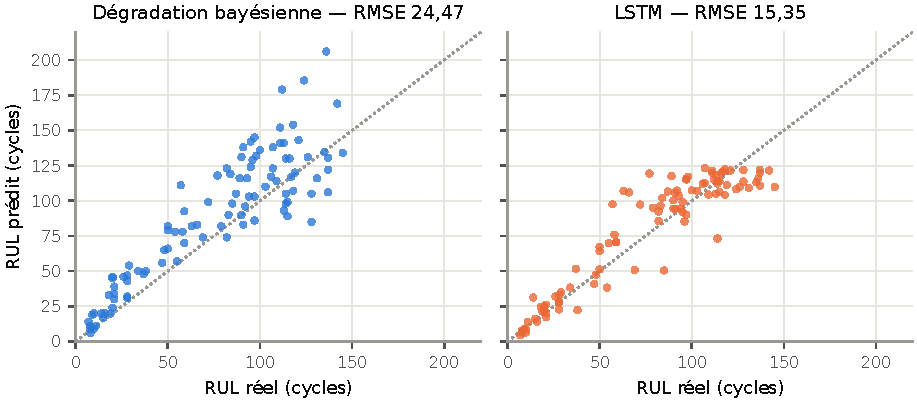
\includegraphics[width=1\linewidth]{figures/rul_predit_vs_reel.pdf}
\caption{RUL prédit en fonction du RUL réel pour les deux modèles ; la diagonale correspond à une prédiction parfaite.}\label{fig:rul_predit_vs_reel}
\end{figure}

\begin{figure}[htbp]
\centering
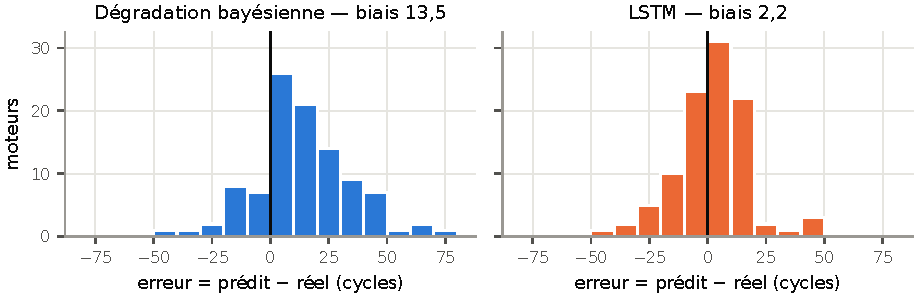
\includegraphics[width=1\linewidth]{figures/rul_erreurs.pdf}
\caption{Distribution des erreurs de prédiction ; une erreur positive est une prédiction tardive.}\label{fig:rul_erreurs}
\end{figure}

La figure~\ref{fig:rul_flotte} présente les prédictions pour l'ensemble de la flotte, triée par RUL réel croissant. Pour les moteurs proches de la défaillance, les deux modèles sont précis et les intervalles du modèle de dégradation sont étroits ; pour les moteurs encore jeunes, l'incertitude augmente fortement.

\begin{figure}[htbp]
\centering
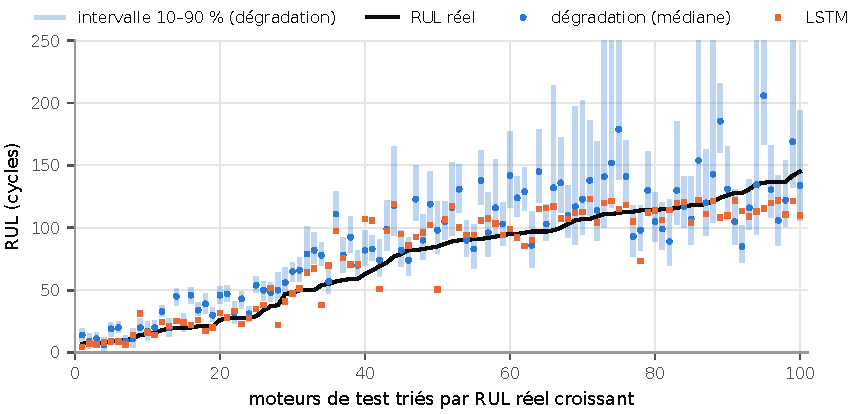
\includegraphics[width=1\linewidth]{figures/rul_flotte.pdf}
\caption{Prédictions des deux modèles pour les moteurs de test triés par RUL réel, avec l'intervalle P10–P90 du modèle de dégradation.}\label{fig:rul_flotte}
\end{figure}

\subsection{Calibration du modèle de dégradation}

Le tableau~\ref{tab:rul_calibration} et la figure~\ref{fig:rul_calibration} évaluent les intervalles de prédiction. À tous les niveaux, la couverture observée est inférieure au niveau nominal : 35 \% pour l'intervalle P25–P75, 54 \% pour P10–P90 et 59 \% pour P05–P95. \textbf{Les intervalles sont trop étroits}, c'est-à-dire que le modèle sous-estime son incertitude.

\begin{table}[htbp]
\centering\small
\begin{adjustbox}{max width=\linewidth,center}
\begin{tabular}{lrrr}
\toprule
Intervalle & Niveau nominal & Couverture observée & Largeur moyenne \\
\midrule
P25 – P75 & 50 \% & 35 \% & 21,7 cycles \\
P10 – P90 & 80 \% & 54 \% & 44,9 cycles \\
P05 – P95 & 90 \% & 59 \% & 65,0 cycles \\
\bottomrule
\end{tabular}
\end{adjustbox}
\caption{Calibration des intervalles du modèle de dégradation}\label{tab:rul_calibration}
\end{table}

\begin{figure}[htbp]
\centering
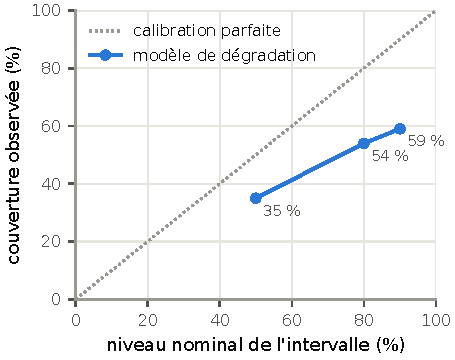
\includegraphics[width=0.55\linewidth]{figures/rul_calibration.pdf}
\caption{Calibration des intervalles du modèle de dégradation : couverture observée en fonction du niveau nominal.}\label{fig:rul_calibration}
\end{figure}

Le tableau~\ref{tab:rul_biais_tranches} détaille le biais selon le RUL réel. Le biais est positif dans toutes les tranches, avec un maximum de +21,4 cycles dans la tranche intermédiaire. Pour les moteurs dont le RUL réel est le plus grand, le biais est plus faible (+7,4) et la couverture meilleure (79 \%), car les intervalles y sont beaucoup plus larges. Le biais médian vaut +11,5 cycles. À titre de diagnostic seulement, l'écart-type des erreurs vaut 20,4 cycles : c'est l'erreur qui resterait si le biais moyen était retiré. Ce n'est pas une performance atteignable, car le biais est mesuré sur le jeu de test lui-même.

\begin{table}[htbp]
\centering\small
\begin{adjustbox}{max width=\linewidth,center}
\begin{tabular}{lrrrr}
\toprule
RUL réel & Moteurs & Biais moyen & MAE & Couverture 10–90 \% \\
\midrule
0 – 50 cycles & 33 & +11,5 & 11,7 & 42 \% \\
50 – 100 cycles & 34 & +21,4 & 23,0 & 41 \% \\
> 100 cycles & 33 & +7,4 & 22,2 & 79 \% \\
\bottomrule
\end{tabular}
\end{adjustbox}
\caption{Biais du modèle de dégradation selon le RUL réel}\label{tab:rul_biais_tranches}
\end{table}

\subsection{Apprentissage du LSTM et exemple d'un moteur}

L'apprentissage du LSTM (figure~\ref{fig:rul_apprentissage_lstm}) s'arrête au bout de 59 époques ; l'arrêt précoce conserve les poids de la meilleure époque (RMSE de validation 13,41 cycles, sur la cible plafonnée). Les erreurs d'entraînement et de validation restent proches, sans signe de sur-apprentissage marqué.

\begin{figure}[htbp]
\centering
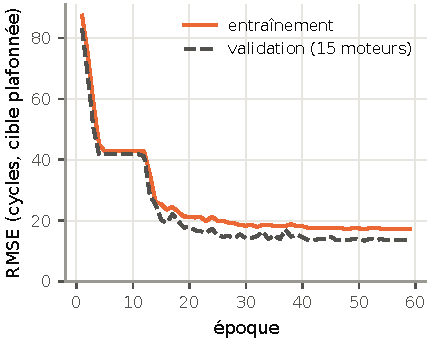
\includegraphics[width=0.55\linewidth]{figures/rul_apprentissage_lstm.pdf}
\caption{Courbes d'apprentissage du LSTM : RMSE d'entraînement et de validation par époque.}\label{fig:rul_apprentissage_lstm}
\end{figure}

La figure~\ref{fig:rul_exemple_moteur} illustre le fonctionnement des deux modèles sur le moteur de test n° 31, observé pendant 196 cycles et dont le RUL réel au dernier cycle est de 8 cycles. Au fil des cycles, les deux prédictions se rapprochent du RUL réel. Au dernier cycle, le modèle de dégradation prédit 9 cycles (intervalle P10–P90 de 3 à 15) et le LSTM 7 cycles. La projection de l'indicateur de santé montre comment le modèle bayésien déduit le RUL du franchissement du seuil.

\begin{figure}[htbp]
\centering
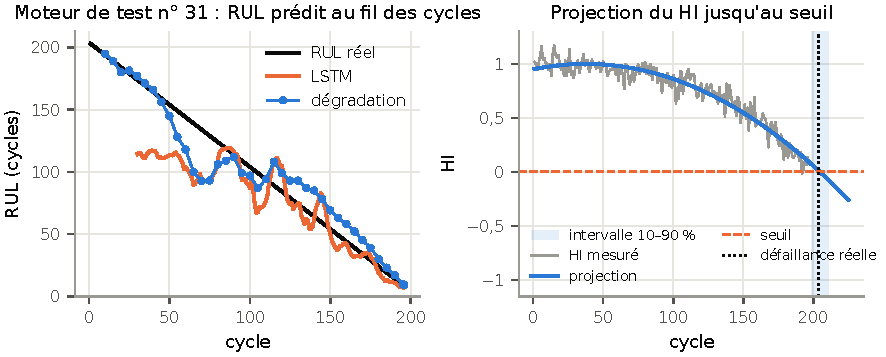
\includegraphics[width=1\linewidth]{figures/rul_exemple_moteur.pdf}
\caption{Moteur de test pris en exemple : RUL prédit à chaque cycle par les deux modèles (gauche) et projection de l'indicateur de santé jusqu'au seuil de défaillance (droite).}\label{fig:rul_exemple_moteur}
\end{figure}

\section{Comparaison des méthodes}\label{sec:comparaison}

Les deux approches de RUL sont complémentaires :

\begin{itemize}
\item le \textbf{LSTM} est nettement plus précis et quasiment sans biais, ce qui est du même ordre que les réseaux récurrents publiés sur FD001 \cite{zheng2017,ramasso2014}. En revanche, il ne fournit pas d'incertitude, ne peut pas dépasser son plafond et reste peu interprétable ;
\item le \textbf{modèle de dégradation} est moins précis et biaisé vers les prédictions tardives, mais chacune de ses étapes est interprétable (trajectoire de l'indicateur de santé, seuil, loi a priori de flotte), et il fournit une distribution du RUL, même mal calibrée à ce stade.
\end{itemize}

Du côté de la fiabilité, l'approche non paramétrique (Kaplan-Meier, Nelson-Aalen) et l'approche paramétrique (Weibull 3P) concordent sur la forme du taux de défaillance et sur la médiane, ce qui renforce la confiance dans le modèle retenu.

\chapconclusion

La loi de Weibull 3P décrit la fiabilité de la flotte, avec un MTTF de 206,3 cycles. Le classifieur atteint une AUC de 0,991 sur le jeu de test. Pour la durée de vie résiduelle, le LSTM est le plus précis (RMSE de 15,35 cycles), tandis que le modèle de dégradation, moins précis (24,47 cycles), fournit des intervalles encore trop étroits. Le chapitre suivant discute ces résultats.
